% !TeX spellcheck = pt_PT2

\chapter{Estado da Arte} \label{ch:estadodaarte}

O estado da arte apresentado neste capítulo tem como objetivo contextualizar o desenvolvimento de \gls{usv} no panorama atual da robótica marítima. São discutidas as principais soluções de propulsão, desde abordagens baseadas em energias renováveis até plataformas motorizadas de alto desempenho, destacando as respetivas vantagens, limitações e áreas de aplicação. Adicionalmente, é feita uma ponte com o trabalho realizado durante a licenciatura, o qual serviu de base conceptual e experimental para o presente \gls{tfm}. Esta análise fornece o enquadramento necessário para compreender a evolução tecnológica nesta área e justifica as opções adotadas no desenvolvimento do protótipo proposto.

\section{Trabalho Relacionado} 
\label{sec:trabalhorelacionado}

O desenvolvimento de \gls{usv} tem atraído crescente atenção devido à sua relevância em operações de monitorização, recolha de dados e exploração de ambientes marítimos. Estas plataformas permitem realizar missões de forma segura e eficiente em áreas de difícil acesso ou potencialmente perigosas para embarcações tripuladas, constituindo uma solução cada vez mais valorizada em contextos científicos, ambientais e de defesa.  

Entre as alternativas de propulsão destacam-se soluções que dispensam motores convencionais. O \emph{Wave Glider}, desenvolvido pela Liquid Robotics \cite{wave-glider}, utiliza a energia das ondas para se deslocar de forma contínua e passiva, sendo particularmente adequado para missões de longa duração com baixo consumo energético. A Figura~\ref{fig:wave-glider} ilustra o princípio de funcionamento do mecanismo de propulsão por ondas (Figura \ref{fig:wave-glider} (A)) e a estrutura de superfície (Figura \ref{fig:wave-glider} (B)) responsável por garantir flutuabilidade e suporte para a instalação de sensores e antenas.

\begin{figure}[H]
    \centering
    \begin{minipage}{0.45\linewidth}
        \centering
        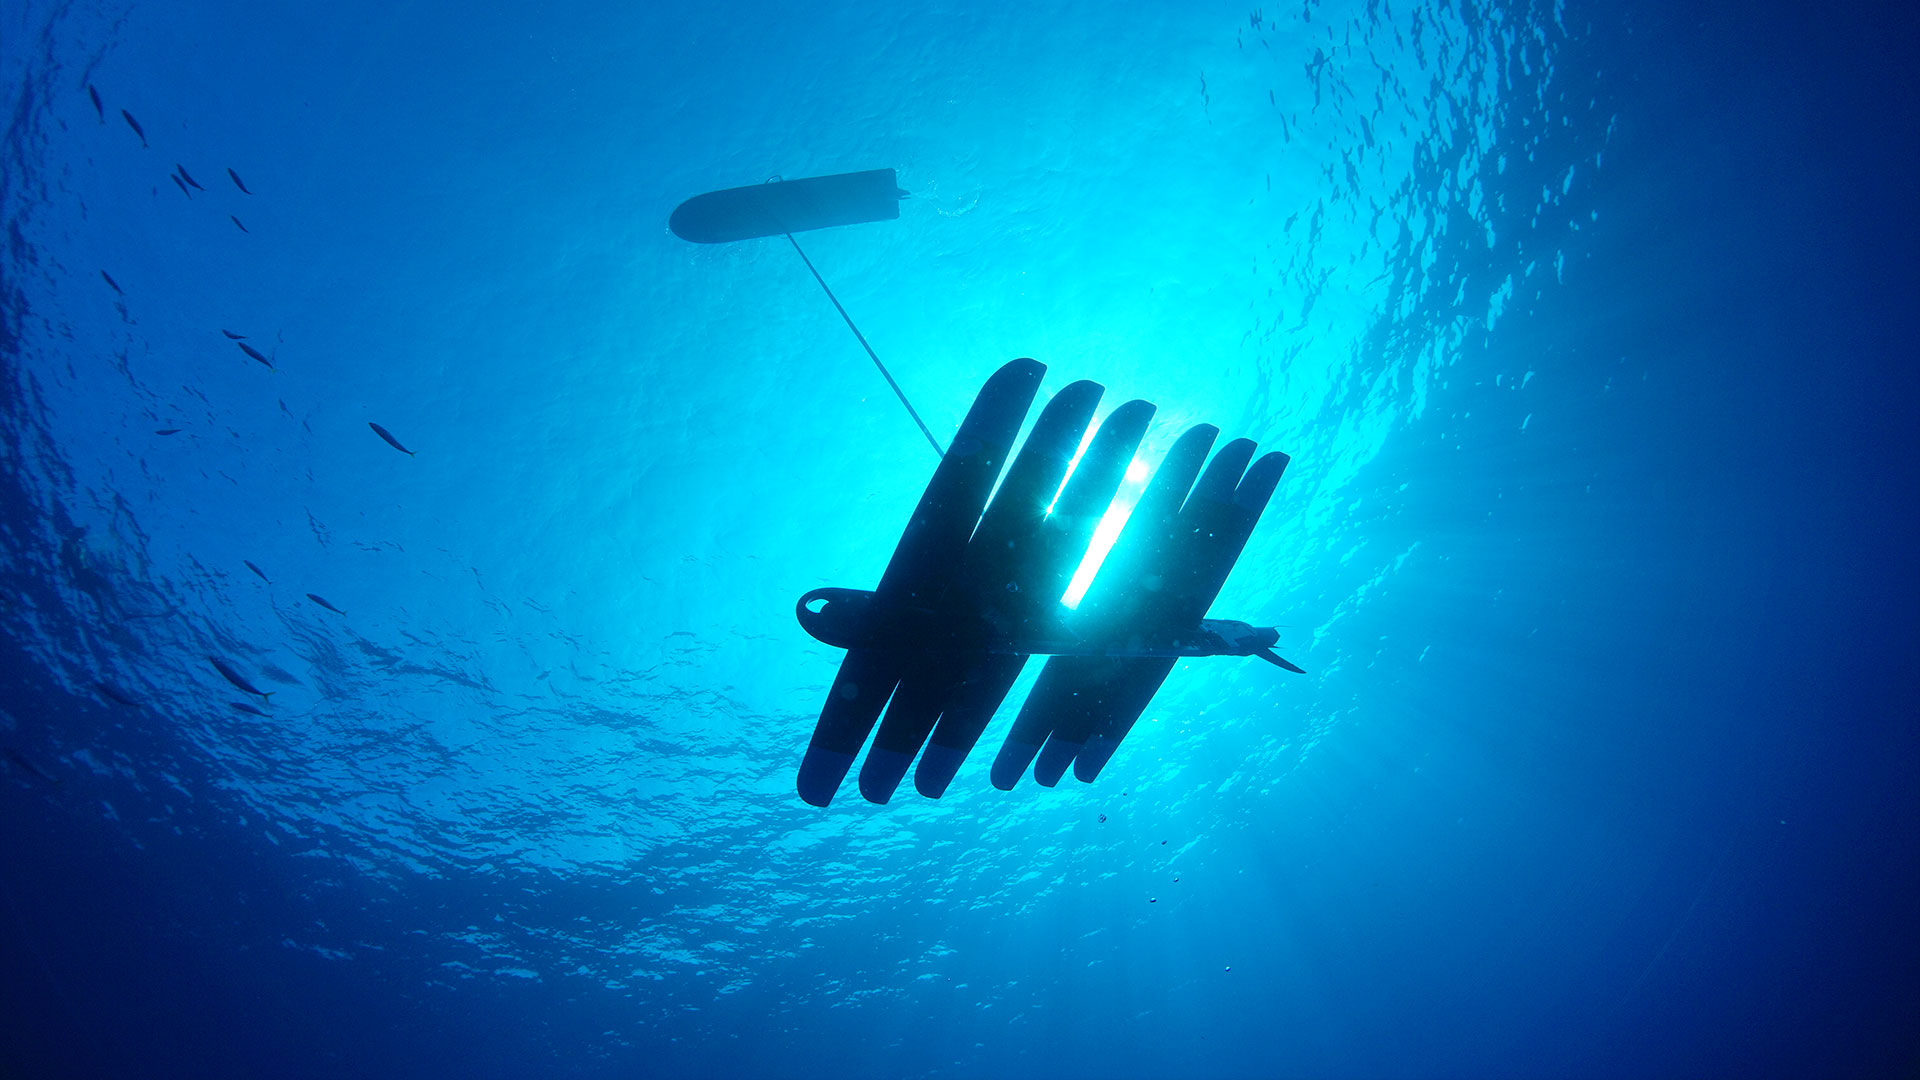
\includegraphics[width=\linewidth]{figuras/wave-glider.jpg}
        \caption*{(A) Mecanismo de propulsão por ondas}
    \end{minipage}
    \hfill
    \begin{minipage}{0.45\linewidth}
        \centering
        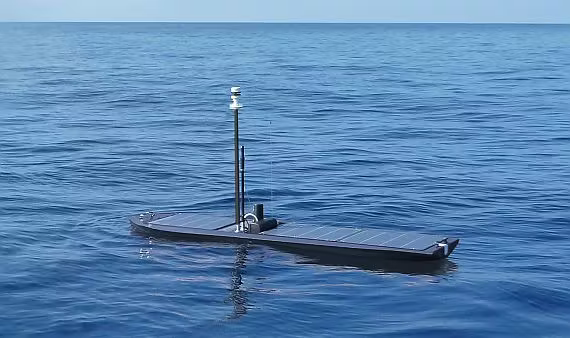
\includegraphics[width=\linewidth]{figuras/wave-glider2.png}
        \caption*{(B) Estrutura da superfície}
    \end{minipage}
    \caption[\gls{usv} Liquid Robotics Wave Glider]{\gls{usv} Liquid Robotics Wave Glider \cite{wave-glider}}
    \label{fig:wave-glider}
\end{figure}

Outra abordagem alternativa é o \emph{Saildrone} \cite{saildrone}, representado na Figura \ref{fig:saildrone}, que recorre à propulsão à vela. 

\begin{figure}[H]
    \centering
    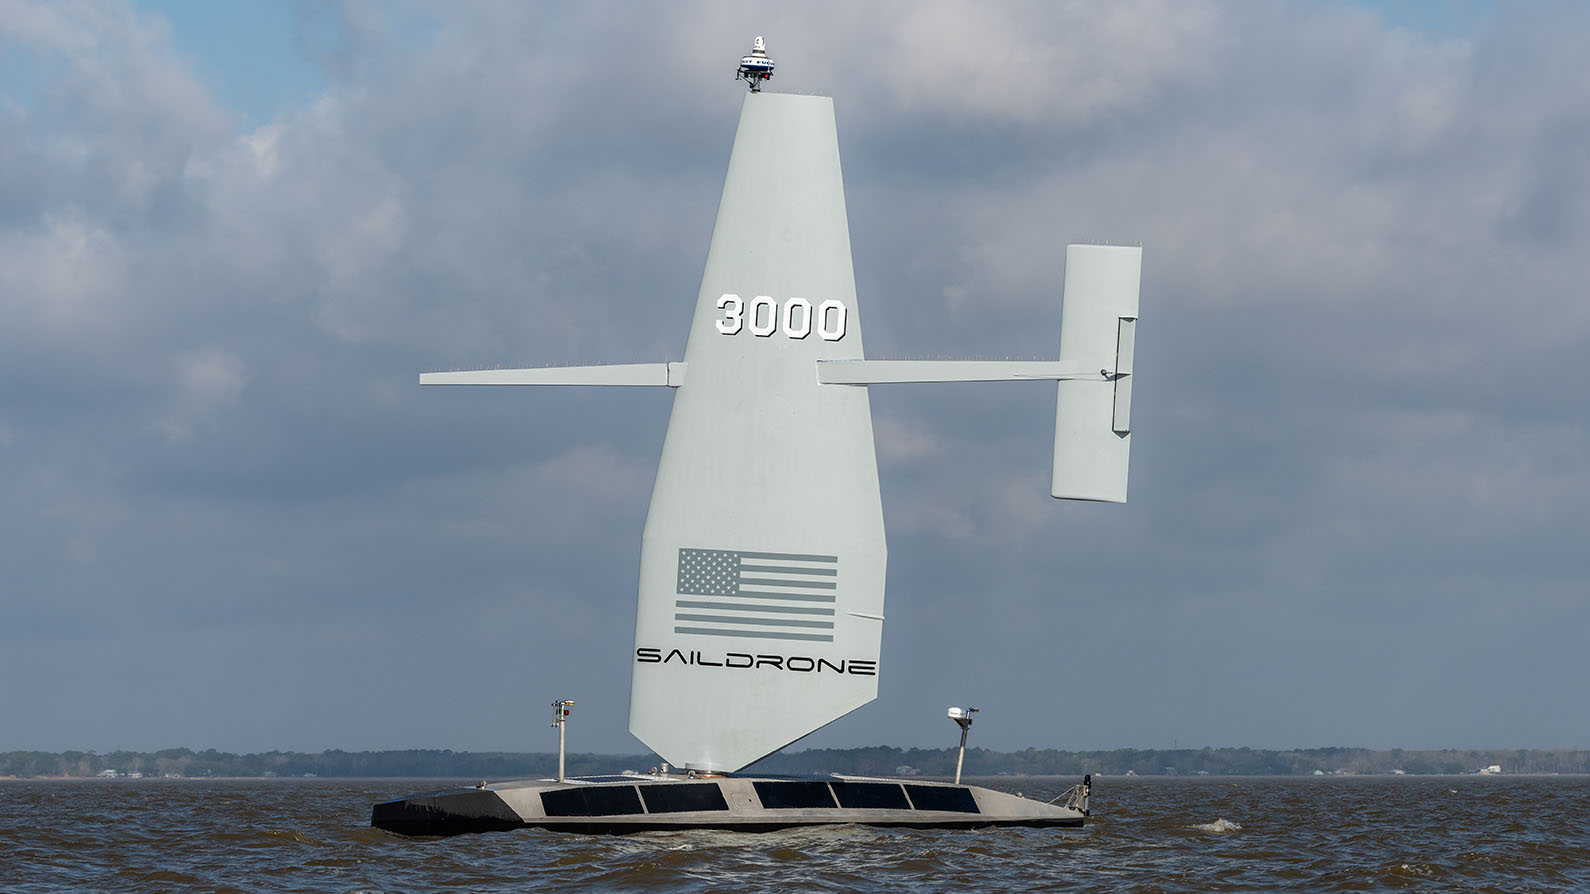
\includegraphics[width=0.5\linewidth]{saildrone-usv.jpg}
    \caption[\gls{usv} Saildrone]{\gls{usv} Saildrone \cite{saildrone}}
    \label{fig:saildrone}
\end{figure}

Este tipo de \gls{usv} tem sido amplamente utilizado em campanhas de monitorização oceânica de larga escala, tirando partido da elevada autonomia oferecida pela energia eólica.  

Apesar das vantagens associadas à utilização de fontes renováveis, as \gls{usv} motorizadas oferecem maior controlo de navegação, velocidade e manobrabilidade, características essenciais em ambientes de correntes variáveis ou condições marítimas adversas. Um exemplo relevante é o SeaRobotics SR-Surveyor \cite{sr-surveyor-class}, amplamente utilizado em levantamentos hidrográficos e mapeamento subaquático, equipado com sonar multifeixe para operações precisas em ambientes costeiros e portuários.  

\begin{figure}[H]
    \centering
    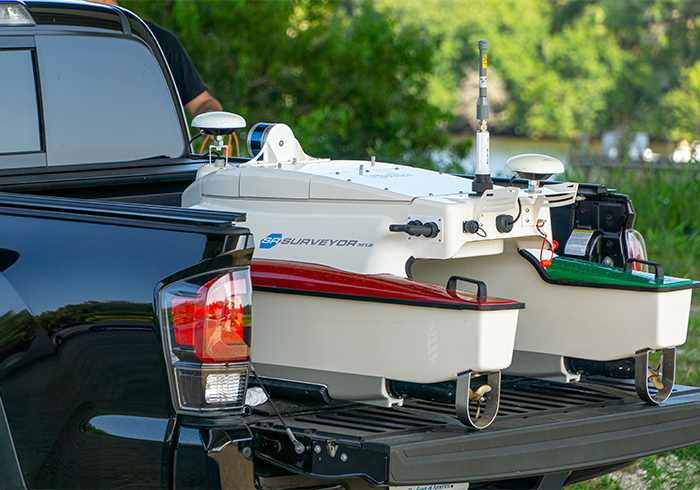
\includegraphics[width=0.5\linewidth]{figuras/sr-surveyorm18-truck-bed.jpg}
    \caption[SeaRobotics SR-Surveyor]{SeaRobotics SR-Surveyor \cite{sr-surveyor-class}}
    \label{fig:sr-surveyor-carrinha}
\end{figure}

A Figura \ref{fig:c-cat-3-asv} apresenta outro exemplo, o \gls{asv} (subclasse de \gls{usv}) Global's C-Cat 3 \cite{c-cat-3-asv}.

\begin{figure}[H]
    \centering
    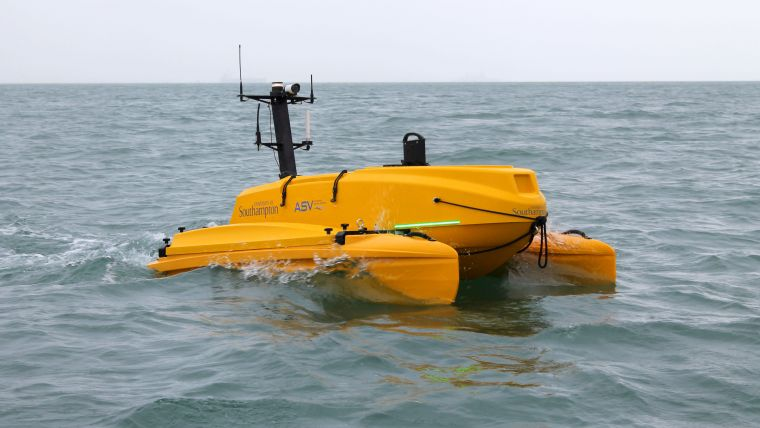
\includegraphics[width=0.5\linewidth]{figuras/c-cat3.jpeg}
    \caption[\gls{asv} Global C-Cat 3]{\gls{asv} Global C-Cat 3 \cite{c-cat-3-asv}}
    \label{fig:c-cat-3-asv}
\end{figure}

O C-Cat~3 \cite{c-cat-3-asv} é um \gls{usv} de dimensões compactas, propulsionado por motor elétrico, projetado para operar em águas pouco profundas. A sua conceção modular e elevada manobrabilidade tornam-no particularmente adequado para missões de monitorização ambiental, levantamentos batimétricos e outras aplicações científicas ou de reconhecimento costeiro.

Também em Portugal têm surgido iniciativas relevantes, como o projeto Sea2Future \cite{sea2future,sea2future2}, desenvolvido pela Escola Superior Náutica Infante D. Henrique, que, conforme ilustrado na Figura \ref{fig:sea2future}, explora o potencial dos \gls{usv} motorizados em cenários de resgate e recolha de dados ambientais.

\begin{figure}[H]
    \centering
    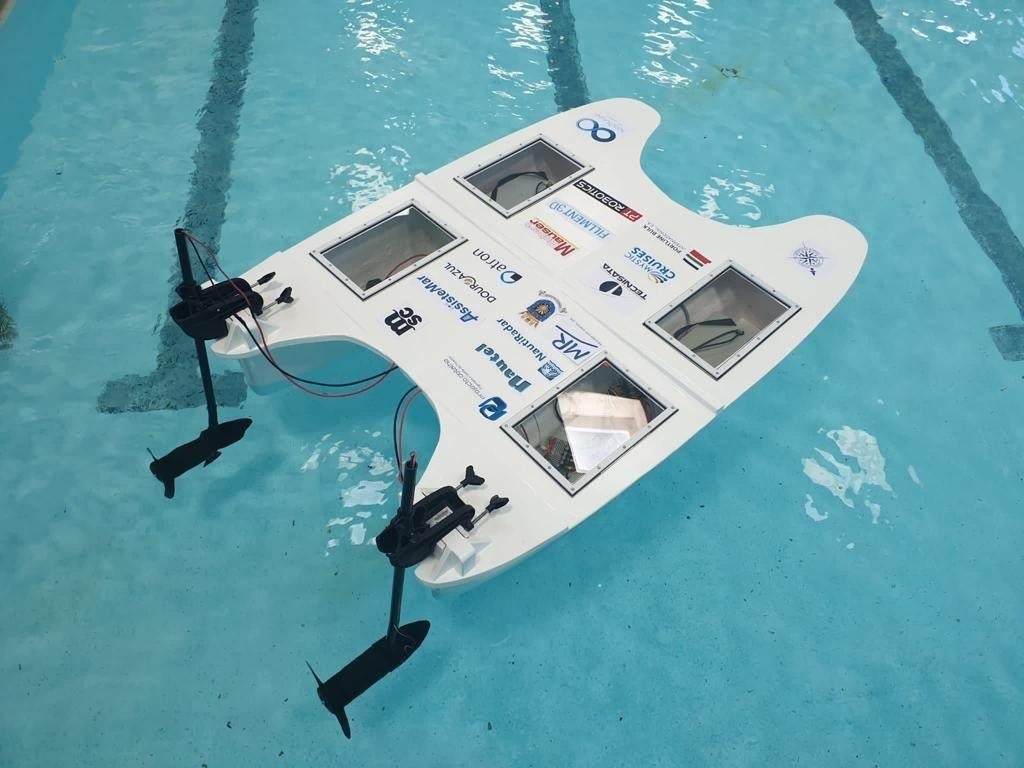
\includegraphics[width=0.5\linewidth]{figuras/sea2future.jpg}
    \caption[\gls{usv} do projeto Sea2Future]{\gls{usv} do projeto Sea2Future \cite{sea2future,sea2future2}}
    \label{fig:sea2future}
\end{figure}

Embora tecnologicamente avançadas, estas soluções comerciais apresentam custos elevados, frequentemente na ordem de centenas de milhares de euros. A aquisição e manutenção de plataformas como o SR-Surveyor ou o C-Cat 3 podem atingir valores próximos de meio milhão de euros, dependendo do conjunto de sensores e da robustez estrutural requerida para operar em ambientes marítimos adversos.  

Nos últimos anos, os avanços tecnológicos em sistemas de controlo e sensorização têm impulsionado o desenvolvimento de \gls{usv} mais acessíveis e modulares. Destaca-se o controlo independente de múltiplos motores, aliado à integração de sensores como \gls{gps}, \gls{imu} e sensores ambientais, que tornam estas plataformas cada vez mais autossuficientes e precisas, abrindo caminho para aplicações em larga escala em monitorização costeira, exploração científica e operações de segurança.

\section{\emph{Background}} 
\label{sec:background}

Durante o percurso académico da licenciatura, foi desenvolvido um projeto descrito em \cite{didactic-robot-thesis}, cujo objetivo principal consistiu na criação de um ambiente didático orientado para a exploração de conceitos fundamentais em robótica, como o controlo de movimento, a comunicação sem fios e a programação em C e Java. O resultado deste trabalho foi um protótipo funcional de robô didático, concebido como uma ferramenta pedagógica eficaz.  

A arquitetura do sistema, apresentada em \cite{didactic-robot-thesis} e ilustrada na Figura \ref{fig:arquitetura-robo-didatico}, foi concebida segundo uma abordagem modular e expansível. Esta estrutura permitia a integração de até quatro motores (localizados na parte direita da figura), incluía os módulos de comunicação (representados no centro) e os módulos de sensorização (à esquerda), possibilitando a implementação e validação de diferentes configurações de forma flexível e adaptável.

\begin{figure}[H]
    \centering
    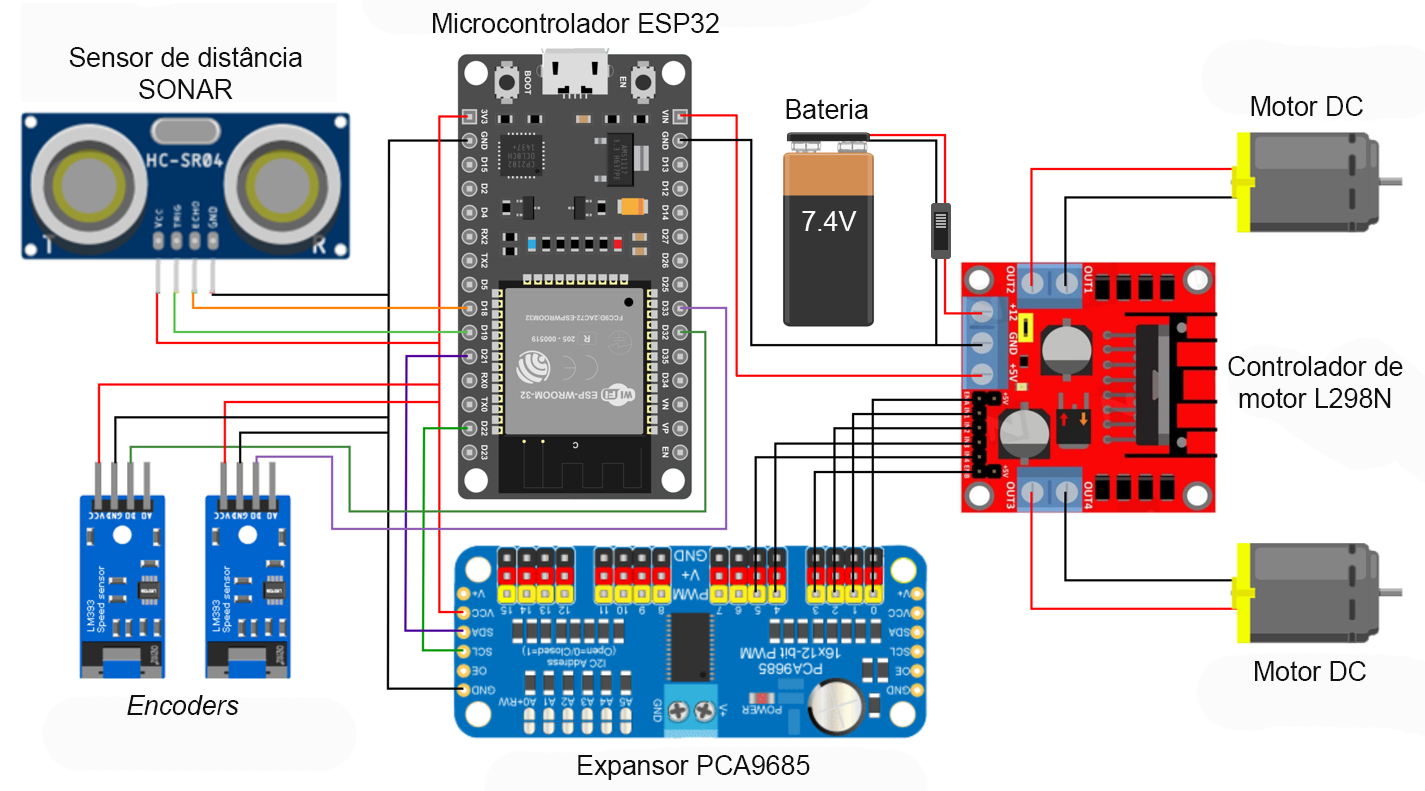
\includegraphics[width=0.95\linewidth]{figuras/arquitetura_robo_didatico.png}
    \caption[Arquitetura do Robô Didático]{Arquitetura do Robô Didático \cite{didactic-robot-thesis}}
    \label{fig:arquitetura-robo-didatico}
\end{figure}

O projeto culminou na construção de um protótipo físico, ilustrado na Figura \ref{fig:estrutura-robo-didatico}, que materializou a arquitetura proposta e demonstrou em ambiente real a integração de motores, sensores e módulos de comunicação. Esta validação experimental confirmou a viabilidade da abordagem modular, destacando a facilidade de substituição ou expansão de componentes.  

\begin{figure}[H]
    \centering
    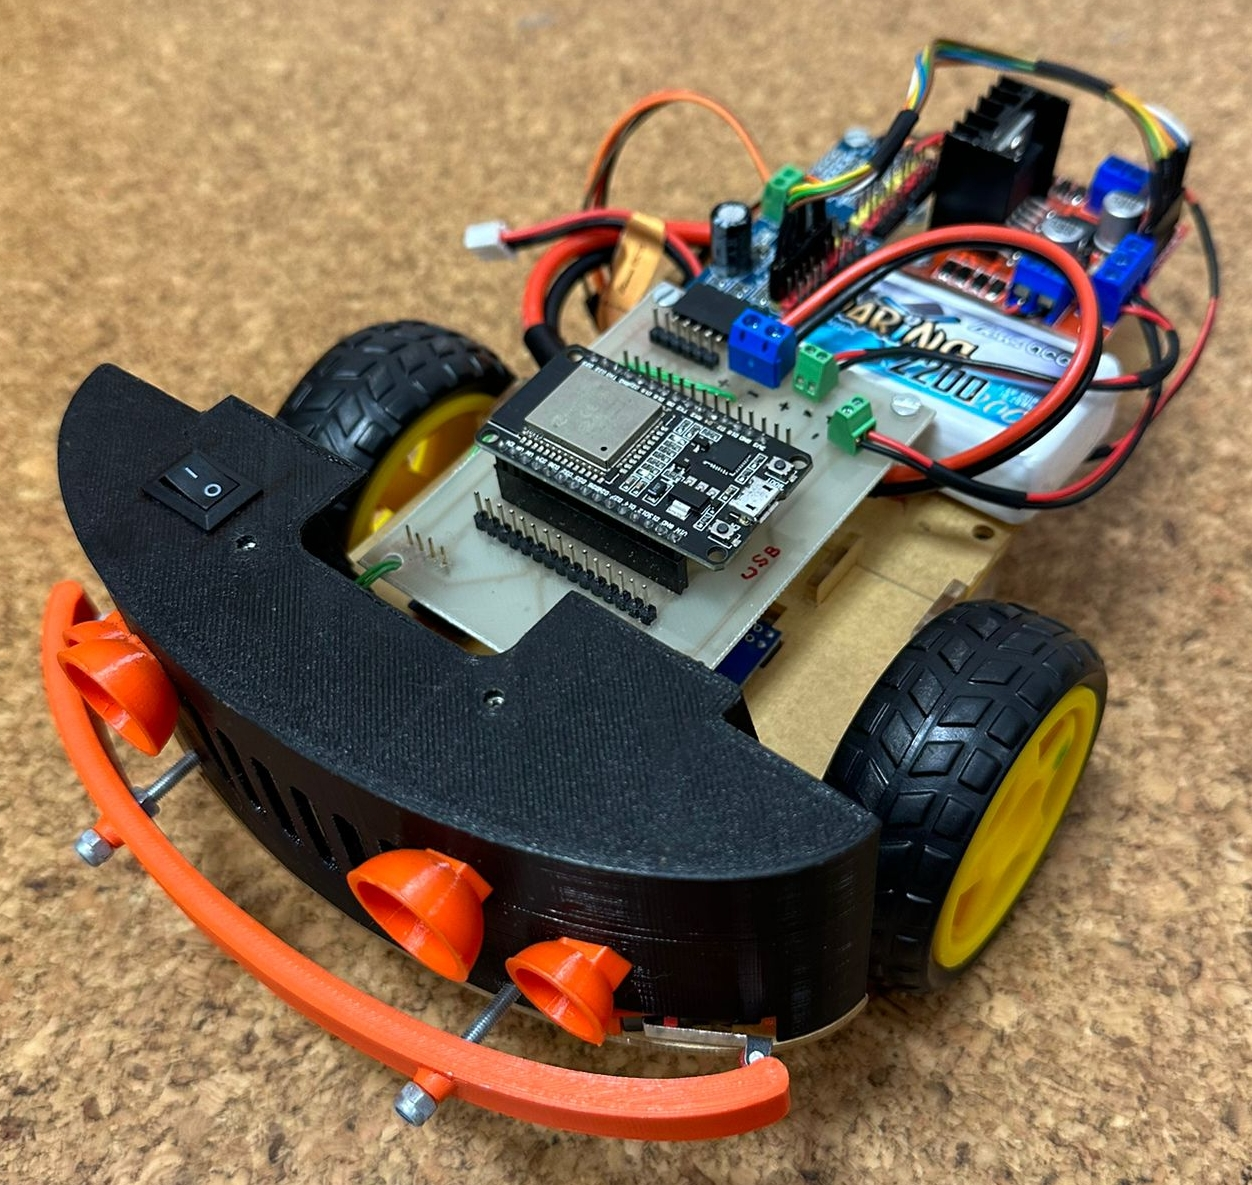
\includegraphics[width=0.5\linewidth]{figuras/robot-didatico.jpg}
    \caption[Estrutura final do Robô Didático]{Estrutura final do Robô Didático \cite{didactic-robot-thesis}}
    \label{fig:estrutura-robo-didatico}
\end{figure}

Um dos elementos centrais desta arquitetura era o controlador de motores, que assegurava a ligação entre a bateria principal e os diferentes atuadores. Este módulo não só suportava uma ampla gama de tensões de entrada, adequada para motores de diferentes características, como também fornecia uma saída regulada para o microcontrolador, simplificando a gestão energética do sistema. A presença de um interruptor dedicado entre a bateria e o controlador permitia desligar rapidamente todo o sistema em situações de teste ou emergência, reforçando a segurança operacional.  

O presente \gls{tfm} surge como uma evolução natural deste projeto, aplicando e expandindo os conceitos adquiridos para o desenvolvimento de um \gls{usv} com capacidade de navegação autónoma. Embora a lógica base da arquitetura tenha sido mantida, nomeadamente a utilização do barramento \gls{i2c} como interface principal de comunicação, foram realizadas adaptações relevantes. Os motores \gls{dc} do robô didático foram substituídos por propulsores \emph{brushless}, controlados por \gls{esc}, mais adequados ao ambiente marítimo.  

Adicionalmente, foram removidos sensores como o sonar e os encoders, que no contexto terrestre permitiam estimar a distância percorrida a partir do número de rotações da roda. No caso de um \gls{usv}, esta abordagem revela-se inviável, pois fatores externos como correntes, vento ou turbulência influenciam a relação entre rotações do propulsor e distância efetivamente percorrida. Para superar esta limitação, os encoders foram substituídos por um \gls{imu} e por um \gls{gps}, que fornecem medições absolutas de aceleração e orientação, permitindo estimar com maior precisão o movimento do veículo em ambiente marítimo.  

Assim, o trabalho desenvolvido na licenciatura serviu de alicerce conceptual e experimental para o presente \gls{tfm}, onde a arquitetura foi adaptada a um contexto mais exigente, integrando sensores e atuadores adequados às particularidades da navegação marítima.
